\documentclass[12pt,a4paper]{article}

\usepackage{graphicx,amsmath,amssymb,float,caption,hyperref,fancyhdr}
\usepackage{newtxtext,newtxmath}
\usepackage{geometry,booktabs,tabularx,array,longtable,microtype}
\usepackage{xcolor}
\usepackage{tikz}
\usetikzlibrary{arrows.meta,positioning,calc}
\geometry{margin=1in}
\setlength{\headheight}{14.5pt}
\pagestyle{fancy}
\fancyhf{}
\lhead{NE39  Five SG + Five IBR  fault + load step}
\rhead{\thepage}
\renewcommand{\headrulewidth}{0.4pt}
\renewcommand{\arraystretch}{1.12}
\emergencystretch=1.5em
\hypersetup{colorlinks=true,linkcolor=blue!45!black,citecolor=blue!45!black,
  urlcolor=blue!45!black}

\DeclareMathOperator{\clamp}{clamp}
\DeclareMathOperator{\sat}{sat}
\newcommand{\pu}{\ifmmode\,\mathrm{p.u.}\else\ p.u.\fi}
\newcommand{\second}{\ifmmode\,\mathrm{s}\else\ s\fi}
\newcommand{\vect}[1]{\boldsymbol{#1}}

% Graphics search path (report lives in docs/source/).
\graphicspath{{figures/}{figures/ne39_5sg5ibr_fault_load/}}
\newcommand{\datadir}{figures/ne39_5sg5ibr_fault_load}
\newcommand{\code}[1]{\texttt{\detokenize{#1}}}

\usepackage{pgfplots,pgfplotstable}
\pgfplotsset{compat=1.18}

\graphicspath{{figures/}{figures/ne39_5sg5ibr_fault_load/}}

\definecolor{pgreen}{RGB}{41,153,69}
\definecolor{pred}{RGB}{191,45,45}
\definecolor{pblue}{RGB}{46,107,191}
\definecolor{pyellow}{RGB}{199,178,38}
\definecolor{pgrey}{RGB}{90,90,90}

\title{\textbf{NE39 Five-SG + Five-IBR Fault and Load-Step Study}\\
\large Five 2-State Classical SGs (Kundur $\delta/\omega$) and Five 17-State Dual-mode-IBR Converters\\[1mm]
\normalsize A Fault + Load-Step Chronology with No SG Tripping}
\author{In-house Power-Flow Project}
\date{13 October 2026}

\begin{document}
\maketitle

\begin{abstract}
This report documents the NE39 (New England IEEE 39-bus) five-plus-five mixed-resource
chronology studied by the project.  Thirty-nine buses carry five synchronous machines
at buses 31, 32, 35, 38, 39 (each a two-state classical plant $\vect x=[\delta,\omega]$)
and five Dual-mode-IBR converters at buses 30, 33, 34, 36, 37 (two GFM, three GFL by a
deterministic design rule).
Because five machines stay online throughout, the synchronous fleet remains the
system voltage/frequency reference at every instant --- so the chronology arms
\emph{no SG breaker event at all}: no SG trip, no SG reclose, and no hand-back
question.  The disturbance is the frozen bus-16 fault ($Z_f=j0.1$~pu,
60--60.15~s) followed by a global $+20\%$ load step at 100~s, horizon 160~s, with
event instants aligned to the delivered 160-s study so the fault windows compare
directly.  MATLAB renders the vector figures and \LaTeX{} typesets the tables, both from
CSV files exported from the stored run artifact, so report tables and figures
share one evidence source.  Failed gates,
refusals, and pending certifications are reported rather than tuned away.
\end{abstract}

\newpage
\tableofcontents
\newpage

\section{Scope, sources and reproduction}\label{sec:scope}

The study system is the TAMU New England 39-bus network with five modelled SGs
(buses 31/32/35/38/39) and five modelled IBRs (buses 30/33/34/36/37).  The whole
system is assembled as a single all-KCL composite differential--algebraic system in
which every SG and every IBR contributes its own differential state block and its own
injection; no device is delegated to an external solver, model, or reference program.

\paragraph{Why no SG trip.}
With five synchronous machines connected, opening any one breaker still leaves four
machines holding the network voltage and frequency reference --- the physical
question the delivered 160-s study answered (``can the converters hold an island
after the machine leaves'') does not arise.  The chronology therefore asks a
different question: \emph{can the mixed fleet ride a bus fault through and absorb a
load step with the machine reference intact?}  Accordingly the profile
\code{fault_load_step} arming fault + load step (and no SG breaker event) was added
to the event schedule, and the catalog row \code{fault_load_step20} freezes its
instants before any result is read.

\paragraph{Figure source and no-synthetic-signal contract.}
The transient figures (Section~\ref{sec:transient}) are rendered from the
accepted trajectory of the stored run artifact, loaded exactly once and exported
as presentation CSV evidence.  Every plotted sample is a raw accepted value;
nothing is smoothed, filtered, decimated, clipped, offset, interpolated, or
augmented with synthetic noise.  Every number in this report is copied from the
stored run or computed from the equilibrium it stores; no gate is relaxed and no
simulation is re-run.

\paragraph{Classification.}
The SG AC/flux equations and the IBR AC/control equations are
\textsf{SOURCE\_MAPPED} or \textsf{PROJECT\_DERIVED} as labelled where they first
appear; machine and converter parameters, per-unit bases, and the disturbance
times are \textsf{CASE\_DEFINED}; the predictor and step-subdivision policy are
\textsf{NUMERICAL\_METHOD}.  The run classification and its
\code{production_certified=false} flag are carried from the manifest and are
not re-decided here.

%=============================================================================
\section{Disturbance chronology}\label{sec:chrono}
%=============================================================================
The scheduled disturbance times are \textsf{CASE\_DEFINED} constants of the
event structure.  Figure~\ref{fig:periods} shows the four operating periods and
the transition instants.  The bus-16 fault is applied at $t=60.000\second$ and
cleared at $t=60.150\second$ (a $0.150$\second fault, impedance
$Z_f=j0.1\pu$); the global load step is applied at $t=100\second$ (every bus load
multiplied by $1+0.2$); the horizon ends at $t=160\second$.  All five SGs are
online at every instant.

\begin{figure}[H]
\centering
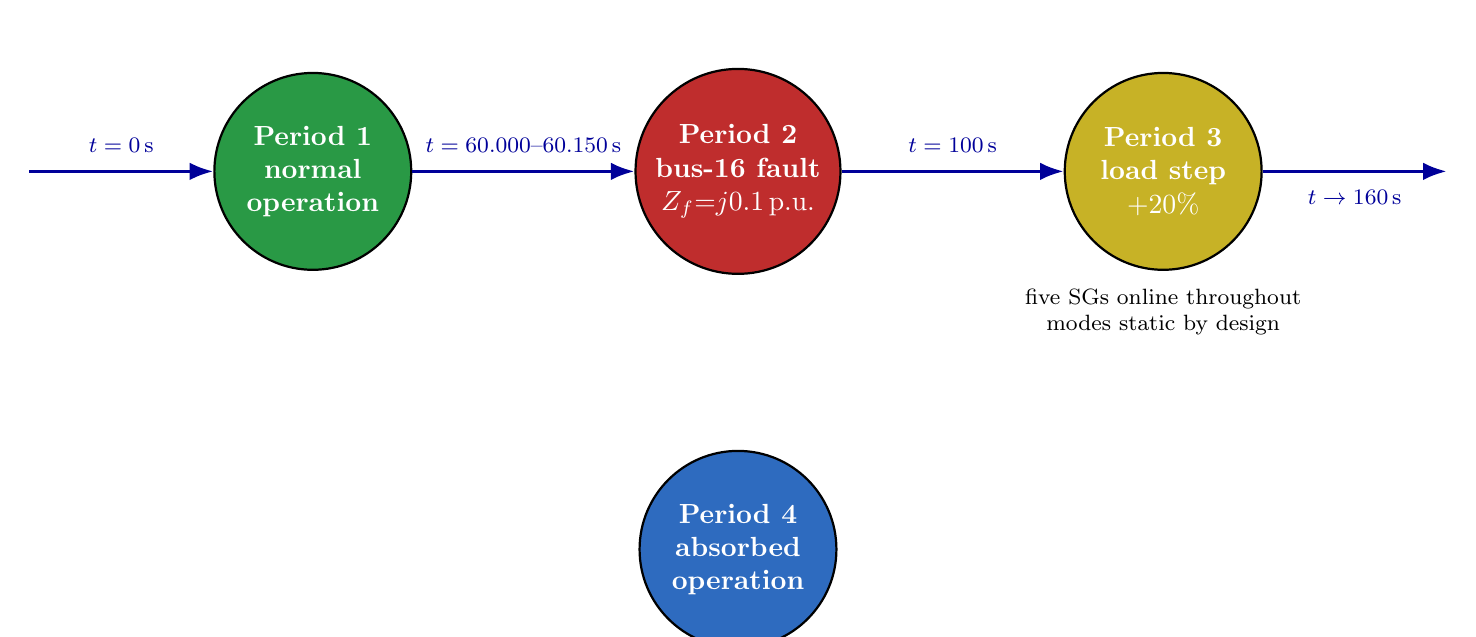
\begin{tikzpicture}[
  font=\normalsize,
  per/.style={circle,draw,thick,minimum size=2.5cm,inner sep=2pt,
    align=center,text=white,font=\bfseries},
  tlab/.style={midway,above=1mm,font=\footnotesize},
  tlabb/.style={midway,below=1mm,font=\footnotesize},
  arr/.style={-{Latex[length=3mm]},very thick,color=blue!60!black}]

\node[per,fill=pgreen] (p1) at (0,0)     {Period 1\\ normal\\ operation};
\node[per,fill=pred]   (p3) at (5.4,0)  {Period 2\\ bus-16 fault\\ $Z_f{=}j0.1\pu$};
\node[per,fill=pyellow](p4) at (10.8,0) {Period 3\\ load step\\ $+20\%$};
\node[per,fill=pblue]  (p5) at (5.4,-4.8){Period 4\\ absorbed\\ operation};

\draw[arr] (-3.6,0) -- node[tlab]{$t=0\second$} (p1);
\draw[arr] (p1) -- node[tlab]{$t=60.000$--$60.150\second$} (p3);
\draw[arr] (p3) -- node[tlab]{$t=100\second$} (p4);
\draw[arr] (p4) -- node[tlabb]{$t\to160\second$} ++(3.6,0);

\node[font=\footnotesize,below=3pt of p4,align=center,text=black]
  {five SGs online throughout\\ modes static by design};
\end{tikzpicture}
\caption{Four-period disturbance chronology.  Green: undisturbed.  Red: the bus-16
fault ridden through with all five machines online.  Yellow: the global $+20\%$
load step.  Blue: the absorbed post-step operation to the horizon.  There is no
SG trip, reclose request, or hand-back period in this chronology.}
\label{fig:periods}
\end{figure}

The products in this report are deliberately separated:
\begin{enumerate}
  \item case inputs (bus dispatch schedules, branch impedances) and the accepted
        initial equilibrium (five SGs synchronous, two IBRs GFM, three GFL);
  \item the 160-\second{} event chronology (fault 60--60.15~s, load step 100~s)
        with \emph{no} mode-change event armed --- initial modes are static by design;
  \item the observed ride-through behaviour: per-device traces and the
        mode/frequency inventory read from the actual histories.
\end{enumerate}

\subsection{Honest status of this run}
\begin{itemize}
\item The run's accepted-path status, sample count, and energy-error integral are
      read from the stored artifact and reported in
      Section~\ref{sec:transient}; they are established from the actual run,
      never asserted.
\item The support supervisor is a no-op \emph{by configuration}
      (\code{automatic_support_supervision=false}): with \code{automatic_gfm_switching=false}
      and no SG breaker event, nothing in the run can change an IBR mode, so there is
      nothing to govern.  Severity/policy evidence is still recorded through
      \code{online_rate_measurement} + \code{ne39_rate_policy} and is reported.
\item Deterministic GFM design rule (PROJECT\_DERIVED): the two largest scheduled
      active powers run GFM (IBR33 at 632~MW, IBR36 at 560~MW), the remaining
      three GFL (IBR30, IBR34, IBR37).  The rule is frozen before any result is
      read and is a study design choice, not a certified dispatch policy.
\item No selector table is built: with five GFM-capable IBRs the exhaustive
      enumeration exceeds its declared bound, and lazy search is a separate
      mission nobody ordered.  The run therefore stays in the
      ``network event, no mode change'' path
      (\code{NETWORK_EVENT_NO_MODE_CHANGE_AUTHORISED}).
\end{itemize}

\section{Automatic GFL/GFM selection: the severity index}\label{sec:sev}

Each IBR carries a two-state supervisor design that decides whether it should behave
as a grid-following current source (GFL) or as a grid-forming voltage source
(GFM).  The decision is driven by a scalar severity $S(t)\in[0,1]$ built from
normalised sub-indices: a voltage-deviation index $J_V$ and a
frequency-deviation index $J_f$, optionally extended by rate-of-change
sub-indices.  In this chronology the supervisor's \emph{decision outputs} are
unused by design (no switching is armed), but the index is still computed and
recorded at every accepted sample --- it is the reported
ride-through-severity evidence of the study.

\paragraph{Sub-indices.}
Let $|V_i(t)|$ be the terminal voltage magnitude of IBR~$i$ and $V_i^{\star}$
the healthy per-bus power-flow magnitude at the five-machine operating point
(Section~\ref{sec:pf}).  Let $f_{\rm coi}(t)$ be the centre-of-inertia
frequency, weighted by each online device's system inertia.  With bases
$\Delta V_{\rm base}=0.10\pu$ and $\Delta f_{\rm base}=0.50$~Hz,
\begin{equation}
  J_V(t)=\frac{\bigl|\,|V_i(t)|-V_i^{\star}\,\bigr|}{\Delta V_{\rm base}},
  \qquad
  J_f(t)=\frac{\bigl|\,f_{\rm coi}(t)-f_0\,\bigr|}{\Delta f_{\rm base}},
  \qquad f_0=60~\mathrm{Hz}.
  \label{eq:jvjf}
\end{equation}

\paragraph{Two-term severity (AGSI).}
The reported severity is the saturated equal-weight average
\begin{equation}
  S(t)=\sat_{[0,1]}\!\Bigl(\tfrac12 J_V(t)+\tfrac12 J_f(t)\Bigr),
  \qquad
  \sat_{[0,1]}(z)=\min\{1,\max\{0,z\}\}.
  \label{eq:agsi}
\end{equation}
$J_V$ responds to a local voltage collapse or overshoot; $J_f$ responds to a
system-wide frequency excursion such as the one the bus-16 fault and the load
step excite.  The equal weighting is a \textsf{PROJECT\_DERIVED}
choice and is frozen before any result is read.

\paragraph{Four-term weighted variant (opt-in).}
The study design also defines an opt-in extension with device-local rate
sub-indices.  With device-local frequency $f_i(t)$, ROCOF
$\dot f_i(t)$, and ROCOV $\dot\nu_i(t)$, and bases
$[\Delta V_{\rm base},\Delta f_{\rm base},\Delta r_{f},\Delta r_{\nu}]
=[0.10\pu,\,0.50~\mathrm{Hz},\,1~\mathrm{Hz/s},\,1~\mathrm{pu/s}]$,
\begin{equation}
\begin{aligned}
  J_{\dot f}(t)&=\frac{|\dot f_i(t)|}{\Delta r_{f}},&
  J_{\dot\nu}(t)&=\frac{|\dot\nu_i(t)|}{\Delta r_{\nu}},\\
  S_{w}(t)&=\sat_{[0,1]}\!\bigl(
      0.35\,J_V+0.35\,J_f+0.15\,J_{\dot f}+0.15\,J_{\dot\nu}\bigr).&&
\end{aligned}
\label{eq:weighted}
\end{equation}
The weights $[0.35,0.35,0.15,0.15]$ and the bases above are
\textsf{PROJECT\_DERIVED, UNVALIDATED} study design: the weighted variant is
armed only when explicitly enabled, and omission keeps the two-term
COI scalar~\eqref{eq:agsi} in force unchanged.  The weights and bases are
validated at option resolution (nonnegative, weights sum to one, positive
bases), and the healthy-PF reference must match each device's bus uniquely ---
otherwise the weighted sample is refused as invalid evidence, never silently
given a guessed reference.

\paragraph{Why $[0.35,0.35,0.15,0.15]$.}
The voltage and frequency deviations $J_V,J_f$ are the two quantities the
supervisor can trust at every instant: each is normalised by a declared base
($\Delta V_{\rm base}=0.10$~pu, $\Delta f_{\rm base}=0.50$~Hz) taken from the
same study design, so they enter the severity with equal standing and share
$0.35+0.35=0.70$ of the total weight.  The rate sub-indices $J_{\dot f},
J_{\dot\nu}$ are supporting evidence only: their bases ($1$~Hz/s, $1$~pu/s)
are design orders of magnitude rather than measured envelopes, their raw
signals are noisier (finite-difference of the accepted samples), and neither
corresponds to a gate the supervisor owns.  They therefore carry the remaining
$0.15+0.15=0.30$, enough to sharpen the trigger during fast transients without
ever outweighing the two primary deviations.  The split is a
\textsf{PROJECT\_DERIVED} study choice --- 70/30 between level and rate
information --- frozen before any result was read, and it is not a certified
or grid-code weighting.

\paragraph{Hysteresis, dwell, and the gates the index does not replace.}
A bare threshold on $S$ would chatter.  The supervisor design therefore uses an
asymmetric two-level comparator with minimum dwell times,
\begin{equation}
  \begin{aligned}
    \text{GFL}\to\text{GFM}:&\quad S\ge\Gamma_{\rm on}=0.65
       \ \text{held for}\ T_{d,\rm on}=0.10\second,\\
    \text{GFM}\to\text{GFL}:&\quad S\le\Gamma_{\rm off}=0.35
       \ \text{held for}\ T_{d,\rm off}=1.00\second.
  \end{aligned}
  \label{eq:hyst}
\end{equation}
The gap $\Gamma_{\rm on}>\Gamma_{\rm off}$ is the hysteresis band.  Thresholds
and dwell times resolve as one contract: when the same scalar is supplied
through two spellings and they disagree, the run fails closed instead of picking
one.  In this chronology the comparator is \emph{recorded but never applied} ---
no switching event is armed, so the severity index and its hysteresis never gate
any transaction, and the diagnostic SCR of Section~\ref{sec:transient} never
enters it either.

\section{Case data and index maps}

\subsection{System and resource map}

The network is the 100-MVA, 60-Hz TAMU New England 39-bus data set.  The
source archive is transcribed with SHA-256 recorded in the case struct; the
project adds the composition (five classical SGs, five Dual-mode-IBR converters,
slack at bus~31 held at $V=1\angle 0^\circ$~pu) and the converter ratings.  The
mixed resource map is
\begin{center}\footnotesize
\begin{tabular}{ccllc}
\toprule
Device index & Bus ID & Device & Model & Initial mode\\
\midrule
1--5  & 31, 32, 35, 38, 39 & SG31--SG39 & \code{sg_classical} (2 states) & synchronous\\
6--10 & 30, 33, 34, 36, 37 & IBR30--IBR37 & \code{Dual-mode-IBR} (17 states) & 2 GFM / 3 GFL\\
\midrule
\multicolumn{4}{r}{Runtime dynamic inventory} & \multicolumn{1}{c}{$5(2)+5(17)=95$}\\
\bottomrule
\end{tabular}
\end{center}

\paragraph{IBR parameters at each bus.}  All five converters share the
Dual-mode-IBR plant constants ($L_f=0.15$~pu, $R_f=0.015$~pu,
$C_{dc}=0.0237216$~pu, $V_{dc,\rm ref}=1$~pu, $M=3.3209$~s,
$D_v=33.2095$~pu, $\tau_E=0.4$~s, $k_Q=0.2$, $k_E=8$, $k_{pV}=1.2$,
$k_{iV}=3.2587$; GFL PLL $k_p=1.2$, $k_i=5$) and differ only in their port
rating and duty:
\begin{center}\footnotesize
\begin{tabular}{crrrrr}
\toprule
Device & Bus & $S_{\rm rating}$ pu & Schedule $P$ pu & \multicolumn{2}{c}{Initial mode}\\
\midrule
IBR30 & 30 & 44.000 & 2.500 & GFL & (100$\times$ schedule: 250~MW)\\
IBR33 & 33 & 36.700 & 6.320 & \textbf{GFM} & (632~MW)\\
IBR34 & 34 & 11.800 & 5.080 & GFL & (508~MW)\\
IBR36 & 36 & 35.300 & 5.600 & \textbf{GFM} & (560~MW)\\
IBR37 & 37 & 18.200 & 5.400 & GFL & (540~MW)\\
\midrule
\multicolumn{3}{r}{Total converter schedule $P$} & \multicolumn{2}{c}{24.900}\\
\bottomrule
\end{tabular}
\end{center}
The P schedule is the rating-proportional dispatch of the composition
contract.  Current limits are $I_{max}^{SS}=I_{max}^{F}=1.2\pu$ device base with
$E_{\rm max}=1.2$, $E_{\rm min}=0.8\pu$, and the fault contract is balanced
positive-sequence RMS with GFM current circles.

\paragraph{SG fleet.}  The five classical machines keep the TAMU GENROU-derived
classical reduction: each carries $x=[\delta,\omega]$ with inputs $[P_m,E_{mag}]$,
$H$ and $D$ from the system-base reduction, $X'$ from the source machine data.
Bus~31 is the declared slack ($V=1$~pu, $0^\circ$); buses 32, 35, 38, 39 are PV
in the composition's operating point.  Because the machines never trip, the
classical plant here needs no governor/excitation/PLL reclose states --- the
two-state form is the study's declared model, not a hidden reduction of a
larger one.

Algebraic voltage order is
\[
\vect y=[V_{x,1},V_{y,1},V_{x,2},V_{y,2},\ldots,V_{x,39},V_{y,39}]^{\mathsf T},
\qquad V_k=V_{x,k}+jV_{y,k},
\]
78 algebraic variables for 39 buses.

\subsection{Bus input data}

\begin{table}[H]\centering\footnotesize
\caption{Case bus data.  These are inputs, not solved PF results: the load
schedules $P_d$/$Q_d$ and shunt admittances $G_s$/$B_s$ straight from the
composition, per unit on the 100-MVA base.}
\pgfplotstabletypeset[col sep=comma,
 columns={bus_id,type,Pd_pu,Qd_pu,Gs_pu,Bs_pu},
 columns/bus_id/.style={column name=Bus},columns/type/.style={column name=Role,string type},
 columns/Pd_pu/.style={column name=$P_L$ pu,fixed,fixed zerofill,precision=3},
 columns/Qd_pu/.style={column name=$Q_L$ pu,fixed,fixed zerofill,precision=3},
 columns/Gs_pu/.style={column name=$G_s$ pu,fixed,fixed zerofill,precision=3},
 columns/Bs_pu/.style={column name=$B_s$ pu,fixed,fixed zerofill,precision=3},
 every head row/.style={before row=\toprule,after row=\midrule},every last row/.style={after row=\bottomrule}]
{\datadir/case_bus_data.csv}
\end{table}

\begin{table}[H]\centering\footnotesize
\caption{Case branch series and charging data in source row order (46 branches,
per unit on the 100-MVA base).}
\pgfplotstabletypeset[col sep=comma,
 columns={branch_index,from_bus,to_bus,r_pu,x_pu,b_pu},
 columns/branch_index/.style={column name=Index},columns/from_bus/.style={column name=From},
 columns/to_bus/.style={column name=To},columns/r_pu/.style={column name=$r$ pu},
 columns/x_pu/.style={column name=$x$ pu},columns/b_pu/.style={column name=$b_c$ pu},
 columns/r_pu/.append style={fixed,fixed zerofill,precision=3},
 columns/x_pu/.append style={fixed,fixed zerofill,precision=3},
 columns/b_pu/.append style={fixed,fixed zerofill,precision=3},
 every head row/.style={before row=\toprule,after row=\midrule},every last row/.style={after row=\bottomrule}]
{\datadir/case_line_data.csv}
\end{table}

The TAMU source leaves bus base kV unspecified (both the source column and
the raw recorder constants), so this report publishes no kV column rather than
inventing one.  All per-unit quantities use the 100-MVA system base.

\section{Common frames, signs, and per-unit conversion}

Every device uses generator sign: positive complex power is injected into the
network,
\[
S=P+jQ=V I^*,\qquad I_{bus}=\sum_{d\in bus} I_d.
\]
Each Dual-mode-IBR converter carries its own local reference (\S\ref{sec:ibr}); the
network-to-device transform is
\begin{align}
v_d&=V_x\cos\delta_{PLL}+V_y\sin\delta_{PLL},\\
v_q&=-V_x\sin\delta_{PLL}+V_y\cos\delta_{PLL},
\end{align}
so device currents rotate back as
$i_x=i_d\cos\delta_{PLL}-i_q\sin\delta_{PLL}$ and
$i_y=i_d\sin\delta_{PLL}+i_q\cos\delta_{PLL}$.  Converter and SG per-unit
values share the 100-MVA system base ($\kappa=S_{base}/M_{base}$ with
$M_{base}=S_{base}$ for the Dual-mode-IBR plant here).

\section{Composite network DAE}

Every device supplies a differential right-hand side and a positive complex
current injection.  The composite equations are
\begin{align}
\dot{\vect x}&=\vect f(\vect x,\vect y,\vect u;\sigma),\\
\vect 0&=\vect g(\vect x,\vect y,\vect u;\sigma)
          =\mathcal R\!\left(Y(\sigma)V-I_{bus}(\vect x,\vect y,\vect u;\sigma)\right),
\end{align}
each on its own numbered line,
where $\mathcal R(z)=[\Re z_1,\Im z_1,\ldots]^{\mathsf T}$ and $\sigma$
contains topology, breaker status, and device mode.  The network admittance
stamps each branch as
\[
Y_{ii}\mathrel{+}=y_s/(a a^*)+jb_c/2,\quad
Y_{jj}\mathrel{+}=y_s+jb_c/2,\quad
Y_{ij}\mathrel{-}=y_s/a^*,\quad
Y_{ji}\mathrel{-}=y_s/a,
\]
with $y_s=1/(r+jx)$, off-nominal ratio $a=\tau e^{j\phi}$, plus the load
admittance fold $Y_{\rm load}=\operatorname{diag}(\overline{\vect S_0}/|\vect V_{pf}|^2)$
from the PF seed.  At the declared reference bus (bus~31), the appropriate KCL
rows are replaced by explicit voltage constraints; the replacement is
metadata-driven.  At the declared load-step instant the same builder stamps the
delta admittance $Y_{\rm step}=0.2\,\operatorname{diag}(\overline{\vect S_0}/|\vect V_{pf}|^2)$:
the step is a genuine network change, not an event-log line.

\section{Synchronous generators: five two-state classical plants}

\subsection{State order and meaning}

\[
\vect x_{SG}=[\delta,\ \omega]^{\mathsf T},
\qquad \vect u_{SG}=[P_m,E_{mag}]^{\mathsf T}.
\]
where $\delta$ is the rotor angle and $\omega$ the per-unit speed in the Kundur
notation ($1.0$ at nominal, absolute), per the two-state classical reduction.
\begin{center}\footnotesize
\begin{tabularx}{\textwidth}{c l l X}
\toprule
Local & State & Unit & Physical meaning\\\midrule
1 & $\delta$ & rad & rotor angle (Kundur) --- electrical internal-EMF angle in the network frame\\
2 & $\omega$ & pu & per-unit rotor speed (absolute; $f=f_0\,\omega$, $1.0$ at nominal)\\
\bottomrule
\end{tabularx}
\end{center}
This is the classical reduction the composition declares: $H$, $D$, $X'$ and the
classical stator-port equation pass through from the source reduction.  The
machines never trip in this chronology, so no governor/excitation/PLL reclose
states exist here.

\subsection{Electrical port and rotor dynamics}

With the series reactance $X'$ and internal EMF
$E=E_{mag}e^{j\delta}$, the injection is
\begin{align}
I&=\frac{E-V}{jX'},\\
P_e&=\operatorname{Re}(V I^*),\\
Q_e&=\operatorname{Im}(V I^*),
\end{align}
and the rotor power balance is energy-consistent in positive speed,
\[
2H\,\omega\,\dot\omega
   =P_m-P_e-D\,\omega(\omega-1),
\]
with $H$ the system-base inertia constant and $D$ the source damping of the
classical reduction.  $P_m$ and $E_{mag}$ are constant inputs during the
chronology: the study design keeps the machine prime-mover and excitation
fixed so the observed ride-through is the network's answer, not the
controllers'.

\section{Dual-mode-IBR converter equations}
\label{sec:ibr}

Each of the five IBRs is a fixed-layout Dual-mode-IBR GFL/GFM superset device with a
shared electrical plant and two distinct controller branches.  The superset
state vector is (17 coordinates when the DC-source current is enabled)
\[
\vect x_{IBR}=[\,i_d,\ i_q,\ V_{dc},\;
\underbrace{\delta_{PLL},\xi_{PLL},\xi_P,\xi_Q,\xi_{id},\xi_{iq}}_{\rm GFL\ controller},\;
\underbrace{\delta_{VSG},\omega_{VSG},E,\xi_{Vd},\xi_{Vq},\xi_{id}^{g},\xi_{iq}^{g}}_{\rm GFM\ controller}\,]^{\mathsf T}
\]
with the active set 10 states in GFL (9 controller + DC source) and 10 in GFM.
Inputs are $\vect u=[P_{\rm ref},Q_{\rm ref},E_{\rm ref}]$.  The source command-delay
states are removed by singular perturbation: the physical actuation delay
$T_d=1.5/f_{sw}\approx0.3$~ms at $f_{sw}=5$~kHz is more than $300\times$ below
the simulation step, so $v_{del}=v_{cmd}$ algebraically.

\subsection{Shared plant: L-filter, DC link, and mode dispatch}

Both branches drive the same physical current and DC-link states:
\begin{align}
\dot i_d&=\frac{\omega_{PLL,pu}L i_q-R i_d+v_{td}-v_d}{L/\omega_b},\\
\dot i_q&=\frac{-\omega_{PLL,pu}L i_d-R i_q+v_{tq}-v_q}{L/\omega_b},\\
P_{ac}&=v_{cd}i_d+v_{cq}i_q,&& \text{(converter-side power)}\\
\dot V_{dc}&=I_{dc,\rm law}(V_{dc},I_{dc},P_{ac}),&& \text{(Thevenin DC source)}
\end{align}
with the non-ideal DC source an EMF behind its internal resistance and an
overvoltage chopper, $I_{dc}=(E_{dc}-V_{dc})/R_{dc}$.

\subsection{GFL branch (9 active controller states)}

In GFL the VSG coordinates are inactive.  With $D_V=v_d^2+v_q^2$,
\begin{align}
\dot\xi_{PLL}&=v_q,\\
\Delta\omega_{PLL}&=k_{p,PLL}v_q+k_{i,PLL}\xi_{PLL},\\
\dot\delta_{PLL}&=\omega_b\Delta\omega_{PLL},\\
i_{d,r}^{\rm raw}&=k_{pP}(P_{\rm ref}-k P_{\rm meas})+k_{iP}\xi_P,\\
i_{q,r}^{\rm raw}&=-(k_{pQ}(Q_{\rm ref}-k Q_{\rm meas})+k_{iQ}\xi_Q),
\end{align}
circularly limited at $I_{max}$ with P-priority, then the inner PI drives the
commanded voltage
\begin{align}
v_{cd}&=v_d+R i_d-\omega_{PLL,pu}L i_q+k_{pI}e_d+k_{iI}\xi_{id},\\
v_{cq}&=v_q+R i_q+\omega_{PLL,pu}L i_d+k_{pI}e_q+k_{iI}\xi_{iq}.
\end{align}

\subsection{GFM branch (10 active controller states)}

In GFM the VSG swing and Q--V voltage-forming dynamics are
\begin{align}
\dot\omega_{VSG}&=\frac{k P_{\rm ref}-P_{\rm meas}-D_v(\omega_{VSG}-1)}{M},\\
\dot\delta_{VSG}&=\omega_b(\omega_{VSG}-1),\\
\dot E&=\frac{k_Q(k Q_{\rm ref}-Q_{\rm meas})-k_E(E-E_{\rm ref})}{\tau_E},
\end{align}
where $E$ is itself the voltage-loop amplitude reference.  The voltage PI
integrators $\xi_{Vd},\xi_{Vq}$ build the current reference from
$(E-v_d,\,0-v_q)$, circularly limited at $I_{max}$, then the same shared
inner current PI and L-filter close the loop.  The anti-windup on the current
clamps is the conditional-hold rule: the integrator holds only when the
limiter is active and its error drives farther outward, with inward recovery
always active.

\subsection{Modes are fixed in this chronology}

Initial modes are fixed at $t=0$ and no event changes them: two converters run
GFM (IBR33, IBR36) and three run GFL (IBR30, IBR34, IBR37) at every instant of
the run, read from the actual mode history.  The mode-transfer machinery of the
plant (runtime transfer preserving $V/I/P/Q$ and $V_{dc}$) is unused here.

\section{How PF, equilibrium, and TS use the equations}\label{sec:tsform}

\subsection{Power flow and the accepted equilibrium}

The source-case PSSE PF is used only to derive the composition's operating
point.  The reported equilibrium instead solves the coupled physical system
\[
\vect f_A(\vect x_0,\vect y_0,\vect u_0)=0,\qquad
\vect g(\vect x_0,\vect y_0,\vect u_0)=0
\]
by Newton on active states plus free algebraic variables, with the physical
all-row KCL gate enforced at $10^{-6}$~pu.  The accepted equilibrium here is
the five-machine composition: converged status, residual, physical-KCL, and
$rcond$ values are read from the stored artifact and reported in
Section~\ref{sec:pf}.  All reported bus, load, branch, and device tables below
share this one voltage vector.  The accepted equilibrium is a
\emph{stationary diagnostic} of the composition \code{case_ne39_5sg_5ibr}: the
TAMU capability contract does not certify a converged Newton solve for this
composition (\code{eq.converged=false} is the case's declared status), and the
residual/KCL levels are the reported truth.

\subsection{Time-domain simulation}

Between event transactions the implicit trapezoidal step solves
\begin{align}
0&=x_{n+1}-x_n-\frac{h}{2}\left[f(x_n,y_n)+f(x_{n+1},y_{n+1})\right],\\
0&=g(x_{n+1},y_{n+1};\sigma_{n+1}),
\end{align}
one equation per line, each numbered,
on the \code{adaptive} stepper with strict LTE control
($\varepsilon_x=2\times10^{-8}$, $\varepsilon_y=2\times10^{-8}$, relative
$10^{-7}$), Newton tolerance $10^{-10}$, step bounds
$dt\in[(0.0025/4096),0.025]$~s, reject limit 16, and no Rannacher arcs.  The
public sampling follows the accepted adaptive steps.  Events are strict
transactions: the handler commits a candidate only after its guard and KCL
checks, and every applied event's pre/right KCL residual is logged
(Table~\ref{tab:events}).

\begin{table}[H]\centering\footnotesize
\caption{Applied event transactions with their physical KCL residuals.}
\label{tab:events}
\pgfplotstabletypeset[col sep=comma,
 columns={event_type,t_s,applied,pre_kcl_norm,right_kcl_norm},
 columns/event_type/.style={column name=Event,string type,string replace*={_}{\_}},
 columns/t_s/.style={column name=$t$ (s),fixed,fixed zerofill,precision=3},
 columns/applied/.style={column name=Applied},
 columns/pre_kcl_norm/.style={column name=pre-KCL (pu),sci,sci zerofill,precision=3},
 columns/right_kcl_norm/.style={column name=right-KCL (pu),sci,sci zerofill,precision=3},
 every head row/.style={before row=\toprule,after row=\midrule},every last row/.style={after row=\bottomrule}]
{\datadir/event_marks.csv}
\end{table}

\section{Accepted equilibrium results}\label{sec:pf}

\subsection{Solved PF figures}

\begin{figure}[H]\centering
\includegraphics[width=\textwidth]{\datadir/matlab_5sg5ibr_pf.pdf}
\caption{Solved equilibrium bus-voltage magnitude and angle at all 39 buses.
Bus 31 is the declared slack at $V=1\angle 0^\circ$~pu; the IBR buses
(30, 33, 34, 36, 37) and the four non-slack SG buses follow the composition's
solved operating point.}
\end{figure}

\subsection{Bus voltages and powers at the accepted equilibrium}

\begin{table}[H]\centering\footnotesize
\caption{Solved bus voltages and bus powers at the accepted five-SG plus
two-GFM equilibrium (per unit on the system base; angles in degrees).}
\pgfplotstabletypeset[col sep=comma,
 columns={bus_id,V_pu,angle_deg},
 columns/bus_id/.style={column name=Bus},
 columns/V_pu/.style={column name=$|V|$ pu,fixed,fixed zerofill,precision=4},
 columns/angle_deg/.style={column name=$\theta$ deg,fixed,fixed zerofill,precision=3},
 every head row/.style={before row=\toprule,after row=\midrule},every last row/.style={after row=\bottomrule}]
{\datadir/normal_pf_bus.csv}
\end{table}

\begin{table}[H]\centering\footnotesize
\caption{Bus generation, load, net injection at the equilibrium (per unit);
the $Q_{shunt}$ column collects charging plus fixed port reactors if present.}
\pgfplotstabletypeset[col sep=comma,
 columns={bus_id,P_gen_pu,Q_gen_pu,P_load_pu,Q_load_pu,P_net_pu},
 columns/bus_id/.style={column name=Bus},
 columns/P_gen_pu/.style={column name=$P_g$ pu,fixed,fixed zerofill,precision=4},
 columns/Q_gen_pu/.style={column name=$Q_g$ pu,fixed,fixed zerofill,precision=4},
 columns/P_load_pu/.style={column name=$P_L$ pu,fixed,fixed zerofill,precision=4},
 columns/Q_load_pu/.style={column name=$Q_L$ pu,fixed,fixed zerofill,precision=4},
 columns/P_net_pu/.style={column name=$P_{net}$ pu,fixed,fixed zerofill,precision=4},
 every head row/.style={before row=\toprule,after row=\midrule},every last row/.style={after row=\bottomrule}]
{\datadir/normal_pf_power.csv}
\end{table}

\subsection{Branch sending-end flows and losses}

\begin{table}[H]\centering\footnotesize
\caption{Branch sending-end flows and losses at the accepted equilibrium.}
\pgfplotstabletypeset[col sep=comma,
 columns={line,from_bus,to_bus,P_from_pu,Q_from_pu,P_loss_pu},
 columns/line/.style={column name=Line},columns/from_bus/.style={column name=From},
 columns/to_bus/.style={column name=To},
 columns/P_from_pu/.style={column name=$P_{from}$ pu,fixed,fixed zerofill,precision=4},
 columns/Q_from_pu/.style={column name=$Q_{from}$ pu,fixed,fixed zerofill,precision=4},
 columns/P_loss_pu/.style={column name=$P_{loss}$ pu,fixed,fixed zerofill,precision=4},
 every head row/.style={before row=\toprule,after row=\midrule},every last row/.style={after row=\bottomrule}]
{\datadir/normal_pf_line_flow.csv}
\end{table}

\subsection{Device injections}

\begin{table}[H]\centering\footnotesize
\caption{Per-device injections at the accepted equilibrium, from each device's
own \code{current_injection} at the stored state (per unit on the system base).}
\pgfplotstabletypeset[col sep=comma,
 columns={device_id,bus_id,mode,P_pu,Q_pu,V_pu},
 columns/device_id/.style={column name=Device,string type},
 columns/bus_id/.style={column name=Bus},
 columns/mode/.style={column name=Mode,string type},
 columns/P_pu/.style={column name=$P_{inj}$ pu,fixed,fixed zerofill,precision=4},
 columns/Q_pu/.style={column name=$Q_{inj}$ pu,fixed,fixed zerofill,precision=4},
 columns/V_pu/.style={column name=$|V|$ pu,fixed,fixed zerofill,precision=4},
 every head row/.style={before row=\toprule,after row=\midrule},every last row/.style={after row=\bottomrule}]
{\datadir/normal_resource_pf.csv}
\end{table}

\section{Event-fence time-domain result}\label{sec:transient}

\subsection{Per-device injections and the grid-strength diagnostic}

At the accepted equilibrium each device's injection is its own
\code{current_injection} at the stored state, $S=V\,i^*$; the per-device
net injections ($P_{\rm inj}$, $Q_{\rm inj}$) are the columns of the
device-injection table above, unchanged.

The grid-strength screen at the same equilibrium is the
\textbf{ASSUMED\_DIAGNOSTIC} short-circuit ratio
\begin{equation}
{\rm SCR}_i=\frac{|V_i|^2}{|Z_{th,ii}|\,S_{{\rm rated},i}},\qquad
Z_{th}=Y^{-1}\ \text{(passive pre-fault network)},
\label{eq:scr}
\end{equation}
where the passive admittance folds the branch series, charging, bus shunts,
and the PF-seed load admittance, and $S_{\rm rated}$ is the composition's
PROJECT\_DERIVED converter rating (the TAMU source leaves no IBR rating).
The computation is a column solve of $Y$ at every IBR PCC, published here only
as a physical grid-strength diagnostic and never a gate outcome.  With four
synchronous machines behind the network at every IBR bus (five minus the slack
contribution at each PCC), the SCR of this composition is structurally higher
than the delivered 160-s study, where the GFM fleet was the only source:
\begin{table}[H]\centering\footnotesize
\caption{ASSUMED\_DIAGNOSTIC grid-strength screen per IBR bus, read from the
stored run's exported evidence (system MVA base).}
\pgfplotstabletypeset[col sep=comma,
 columns={bus_id,abs_Zth_pu,Ssc_MVA,rating_MVA,SCR},
 columns/bus_id/.style={column name=Bus},
 columns/abs_Zth_pu/.style={column name=$|Z_{th}|$ pu,fixed,fixed zerofill,precision=4},
 columns/Ssc_MVA/.style={column name=$S_{sc}$ MVA,fixed,fixed zerofill,precision=1},
 columns/rating_MVA/.style={column name=$S_{\rm rating}$ MVA,fixed,fixed zerofill,precision=1},
 columns/SCR/.style={column name=SCR,fixed,fixed zerofill,precision=2},
 every head row/.style={before row=\toprule,after row=\midrule},every last row/.style={after row=\bottomrule}]
{\datadir/scr_diagnostic.csv}
\end{table}

\subsection{Time-domain result in numbers}

The measured series of the actual run are the exported CSV evidence read
unchanged: per-device power (\code{ts_device_power.csv}), per-device current
(\code{ts_device_current.csv}), frequency traces (\code{ts_device_frequency.csv},
\code{ts_coi_frequency.csv}), the five SG rotor speeds (\code{ts_sg_frequency.csv}),
and the network voltage envelope (\code{ts_bus_vmin_vmax.csv}).  The figures of
this section render those series without modification; every plotted sample is a
raw accepted value of the stored 160-s trajectory, and the fault window
($60\le t<60.15$~s) aligns with the delivered 160-s study at the same instant.

\subsection{Per-device mode, power, and voltage traces}

Figure~\ref{fig:modepq} shows the supervisory state and the per-device
active/reactive power over the full chronology $0\text{--}160\second$: the top
strip is each IBR's grid-forming/grid-following mode (static by design --- no
mode-change event exists), the second strip is the five SG rotor speeds
(all five machines hold the reference throughout), and panels (a)--(b) are
the raw accepted power samples in per unit on the system base.

\begin{figure}[H]\centering
\includegraphics[width=0.94\textwidth]{\datadir/matlab_5sg5ibr_mode_pq.pdf}
\caption{Top strip: grid-forming/grid-following mode of each of the five IBRs
(static by design).  Second strip: the five SG rotor speeds (all five machines
online at every sample).  (a) Per-device active power $P_i$ pu.  (b) Per-device
reactive power $Q_i$ pu.  Raw accepted samples of the stored 160-s trajectory;
$t\in[0,160]\second$ full window.}
\label{fig:modepq}
\end{figure}

Figure~\ref{fig:elec} is the eight-panel electrical response: (a) active power
$P_i$; (b) reactive power $Q_i$; (c) $d$-axis current; (d) $q$-axis current;
(e) device/COI frequency; (f) device terminal voltage; (g) network maximum
voltage; (h) network minimum voltage --- all per unit, all raw accepted samples.

\begin{figure}[H]\centering
\includegraphics[width=0.86\textwidth]{\datadir/matlab_5sg5ibr_electrical.pdf}
\caption{Eight-panel electrical response (raw accepted samples, stored 160-s
trajectory, $t\in[0,160]\second$ full window).  (a) active power $P_i$;
(b) reactive power $Q_i$; (c) $d$-axis current; (d) $q$-axis current;
(e) device/COI frequency; (f) device terminal voltage; (g) network maximum
voltage; (h) network minimum voltage.  One common legend at the top of the
figure identifies every device trace.}
\label{fig:elec}
\end{figure}

Figures~\ref{fig:env}--\ref{fig:dqiq} collect the remaining view families
rendered from the same CSV evidence.

\begin{figure}[H]\centering
\includegraphics[width=0.96\textwidth]{\datadir/matlab_5sg5ibr_envelope.pdf}
\caption{Bus-voltage envelope ($\min_k|V_k|$ to $\max_k|V_k|$) over the full
160-s chronology, with the applied event marks at 60, 60.15, and 100~s.}
\label{fig:env}
\end{figure}

\begin{figure}[H]\centering
\includegraphics[width=0.86\textwidth]{\datadir/matlab_5sg5ibr_envelope_fault.pdf}
\caption{Voltage-envelope detail of the fault window, $t\in[59.4,60.8]\second$.}
\label{fig:envfault}
\end{figure}

\begin{figure}[H]\centering
\includegraphics[width=0.96\textwidth]{\datadir/matlab_5sg5ibr_ts_pages.pdf}
\caption{Time-series family page: (a) device and COI frequency; (b) device
active power (MW); (c) device reactive power (MVAr); (d) device current
magnitude; (e) the five SG rotor frequencies ($f_0\cdot\omega$); (f) device mode
level (0 open / 1 GFL / 2 VF, static here --- no mode-change event exists).}
\label{fig:tspages}
\end{figure}

\begin{figure}[H]\centering
\includegraphics[width=0.96\textwidth]{\datadir/matlab_5sg5ibr_sg_frequency.pdf}
\caption{The five two-state classical SG plants through fault and step: rotor
frequencies $f_0\cdot\omega$ (top) and absolute rotor speed (bottom), read
unchanged from each plant's own state block.}
\label{fig:sgf}
\end{figure}

\begin{figure}[H]\centering
\includegraphics[width=0.96\textwidth]{\datadir/matlab_5sg5ibr_dq_id.pdf}
\caption{Converter $d$-axis current states $i_d$ (device MVA base) of the five
Dual-mode-IBR plants, raw accepted samples.}
\label{fig:dqid}
\end{figure}

\begin{figure}[H]\centering
\includegraphics[width=0.96\textwidth]{\datadir/matlab_5sg5ibr_dq_iq.pdf}
\caption{Converter $q$-axis current states $i_q$ (device MVA base) of the five
Dual-mode-IBR plants, raw accepted samples.}
\label{fig:dqiq}
\end{figure}

\section{Limitations and interpretation}

\begin{itemize}
\item \code{production_certified=false}: no claim in this report is a
      production or hardware certificate.  The run classification is a
      project-derived study.
\item The accepted equilibrium of the five-machine composition is a stationary
      diagnostic with \code{eq.converged=false} (the case's declared TAMU
      capability status); residual and physical-KCL levels are reported as
      measured.
\item The support supervisor is off by configuration; the severity index and
      its hysteresis comparators are recorded but never applied.  No switching
      behaviour can be inferred from this run.
\item The load step is global ($+20\%$ on every bus load), not a per-bus
      staged step --- the study design's declared scope.
\item The GFM/GFL split (two largest scheduled P) is a deterministic design
      rule, not a certified dispatch policy.
\item The converter fault contract is balanced positive-sequence RMS with
      GFM current circles.  It is not an EMT, negative-sequence, or
      zero-voltage model, and it does not reproduce the source GENROU
      fault-current waveform.
\item No kV column is published: the TAMU source leaves bus base kV
      unspecified, and inventing one would be a fabrication.
\item With five machines online the study cannot answer the mode-transfer or
      islanding questions the delivered 160-s study answered --- that is the
      design, not a gap.
\end{itemize}

\section{Conclusion}

The report exposes a traceable chain from the TAMU case inputs through the
accepted five-machine composition equilibrium, the composite DAE, the strict
fault + load-step event chronology, and the observed ride-through behaviour.
The same device equations initialise the equilibrium and are integrated for TS,
the network residual is enforced all-row in both, and the final inventory
(five SGs synchronous, two GFM, three GFL --- unchanged from $t=0$) is read
from the actual mode history and never from a target.  Because five machines
stay the reference, no SG breaker event is armed anywhere in the chronology.
Native \LaTeX{} plots retain the exact stored series at shared typography, and
every refusal --- the unused supervisor, the unconverged equilibrium status ---
remains in the report at the point where it was produced.

\begin{thebibliography}{9}
\bibitem{athay} T. Athay, R. Podmore, and S. Virmani,
``A Practical Method for the Direct Analysis of Transient Stability,''
IEEE Transactions on Power Apparatus and Systems, PAS-98(2), 1979;
attribution follows the TAMU distribution metadata.
\bibitem{pai} M. A. Pai, \emph{Energy Function Analysis for Power System
Stability}, Springer, 1989.
\bibitem{tamu} Texas A\&M University, \emph{New England IEEE 39-Bus System}
distribution, \url{https://electricgrids.engr.tamu.edu/electric-grid-test-cases/new-england-ieee-39-bus-system/}.
\bibitem{eecon49} EECON49 course material, converter block diagram and
parameter table, Eqs.~(6)--(29), Figs.~1--2.
\bibitem{ledesma} Source transcription provenance:
\code{docs/project/NE39_TAMU_MIGRATION.md}.
\end{thebibliography}

\end{document}
